\section{How to Simulate the Rational Programmer} 

Code migration is the raison d'\^etre of Typed Racket, which is why the community
uses ``migratory typing'' instead of gradual typing. Roughly speaking a
programmer uses a gradually typed language to incrementally add types to a code
base. From this perspective, a code base consists of some number of components,
say modules, and a programmer converts a component at a time from its untyped
state to a typed one. 

Based on this idea, a metric for migratory paths is a concise way to
evaluate the effectiveness of a rational programmer. The components of
an ill-typed program, such as one of  our ill-typed mutants, 
create a \emph{debugging scenario space}, a lattice like
the one introduced by ~\citet{tfgnvf-popl-2016} for performance
evaluations. As we discuss briefly at the end of ~\ref{sec:mutate}, 
this space consists of variants of the program, dubbed
\emph{scenarios}, that differ in their type specifications. In the
setting of migratory typing,\footnote{The method can be adapted to
so-called true gradual typing systems~\cite{svcb-snapl-2015} in a
straightforward manner.} each scenario differs from another in which
components are typed. Formally, a program $\system$ is a set of
components $\set{\component}$, and a scenario $\conf$ is a subset of
$\set{\component}$ . These scenarios of $\system$ are ordered by the
subset relation and thus form a lattice $\lattice{\system}$ with
$2^{\size{\system}}$ elements.  The bottom scenario of
$\lattice{\system}$ is always $\emptyset$ and the top one is $\system$
itself. In between are all the mix-typed scenarios.

With these definitions, the actions of the rational programmer map to
an ascending chain---dubbed a \emph{trail}---in $\lattice{\system}$.
The starting scenario $\conf_0$ of a trail---also referred to as the
\emph{root} (of the trail)---is the scenario that the programmer
attempts to debug initially. The easiest scenarios are those that the
type checker rejects outright, because a type error pinpoints an
impedance mismatch between the broken code of one component and its
typed interface to others. At this point, the programmer has
identified the broken component. If the scenario type-checks, the
programmers runs the program until it raises an exception.  The
rational programmer uses the blame assignment\footnote{Blame can
result either directly from a run time type check or, in the absence
of blame, from an exception that we track back to the component that
causes it with the help of the stack trace.} to decide which
component(s) to equip with types. This choice constructs scenario
$\conf_{i+1}$ from $\conf_{i}$ and implies the creation of an
ascending chain.  Intuitively, with each step along the chain, the
rational programmer reduces the current scenario to an ``easier'' one
to debug.

% The successor of a scenario on a trail has more typed component;
% formally, configuration $\conf_{i+1}$ on the trail differs from its
% predecessor $\conf_{i}$ in that more components are typed.

The next three subsections specialize the trail-scenario idea to the
various semantics of gradual typing. Once this machinery is in place,
we use the fourth subsection to state the precise experimental
research questions that correspond to the high-level question on the
first page and to explain our experimental process. The final
subsection extends the development with a discussion of how we can
measure the rational programmer's effort along the trail. 


%% -----------------------------------------------------------------------------
\subsection{Modes of the Natural Rational Programmer} \label{sub:natural}

The natural semantics assigns blame to exactly one boundary.  A blame assignment
has the following specific meaning: the typed component may make incorrect type
assumptions about the untyped component in its interface, or the correct
interface exposes a bug in the untyped component. Our setup rules out the first
alternative (but see section~\ref{sec:conclusion}), and therefore the rational
programmer extends the trail to a scenario that swaps out the untyped component
for its typed counterpart.

We can turn this description into a formal definition of the trail. 
\begin{quote}
\it A \emph{natural blame trail} is a sequence of scenarios $\conf_0,...\conf_n$ of
a program $\system$ such that for all $0 \leq i \leq n - 1$, $\conf_i \subset
\conf_{i+1}$ and $\conf_{i+1} \setminus \conf_i =\{\blame{\system, \conf_i}\}$ where
$\blame{\system, \conf}$ denotes the component that $\conf$ blames.
\end{quote}

When the buggy untyped component of a program is replaced by the typed counterpart,
the type checker fails if this component causes the impedance mismatch. Hence, a
trail that end at an ill-typed scenarios successfully pinpoints the location of
bugs. 
\begin{quote}
\it A natural blame trail $\conf_0,...\conf_n$ in a lattice $\lattice{\system}$ is
\emph{successful} iff its last scenario $\conf_n$ does not type check.  A natural
blame trail $\conf_0,..,\conf_n$ in a lattice $\lattice{\system}$ is \emph{failing}
iff $\conf_n$ type checks and the trail cannot be extended further.
\end{quote}
That is failing natural blame trails are those that have not reached a scenario that
reveals the bug at compile time and their last scenario does not produce blame. Thus
the rational programmer receives no hints from the gradual type system on how to
continue the search for the bug.

Equipped with these preliminary definitions, we can precisely define what it means
for blame to add value to a gradual type system in a specific setting. 
\begin{quote}
\it
Given a program $\system$, natural blame is\\
(1) \emph{always useful} iff $\lattice{\system}$ contains no failing natural blame trails.\\
(2) \emph{sometimes useful} iff $\lattice{\system}$ contains successful natural blame trails.\\
(3) \emph{never useful} iff $\lattice{\system}$ contains no successful natural blame
trails.\\
\end{quote}

While these definitions describe how a rational programmer might gauge whether it
pays off to heed blame assignments during debugging, they do not answer whether
blame is a critical piece of the rational programmer's process.  For instance,
typing a random component might be as useful as typing the blamed one.

To account for this situation, we devise a new mode of the natural rational
programmer that follows a random migration process:
\begin{quote}
\it A natural random trail is a sequence of scenarios $\conf_0,...\conf_n$ of a
program $\system$ such that for all $0 \leq i \leq n - 1$, $\conf_i \subset
\conf_{i+1}$ and $\conf_{i+1} \setminus \conf_i = \{\random{\system, \conf_i}\}$
where $\random{\system, \conf}$ denotes a randomly selected component of $\system$
that is not in $\conf_i$.
\end{quote}
Similar to natural blame we determine how successful the random
migration is based on the success of natural random trails: 
\begin{quote}
\it
Given a program $\system$, natural random blame is\\
(1) \emph{always useful} iff $\lattice{\system}$ contains no failing natural random blame trails.\\
(2) \emph{sometimes useful} iff $\lattice{\system}$ contains successful natural random blame trails.\\
(3) \emph{never useful} iff $\lattice{\system}$ contains no successful natural
random blame trails.\\
\end{quote}

Putting the pieces together, we can now define that blame assignments adds value in
the context of a natural semantics if blame-based migration is better than random
migration.
\begin{quote}
\it Natural blame adds value to natural for a program $\system$ over pure chance iff
  natural blame is more successful than natural random. And, natural blame is more
  successful than natural random for $\system$ if either natural blame is always
  successful for $\system$ when natural random is sometimes or never successful, or
  natural blame is sometimes successful for $\system$ when natural random is never
  successful.
\end{quote}

Even if the success of the natural rational programmer is not by pure chance, it
could well be because the natural semantics perform runtime type checks at the same

%% -----------------------------------------------------------------------------
\subsection{Modes of the Erasure Rational Programmer} \label{sub:erasure}

 Since gradually typed languages with erasure semantics do not come with
 blame assignment, a rational programmer can only hope that the underlying
 safety checks and their exceptions are helpful.  Thus, adapting the
 definitions related to exception and random trails from natural to
 erasure, we characterize when the effect of erasure exceptions in debugging a
 program $\system$ goes beyond that of pure chance. 

\begin{quote}
\it
  Erasure exceptions add value to erasure for a program $\system$ over pure chance
  iff erasure exception is more successful than erasure random.
\end{quote}
\noindent


%% -----------------------------------------------------------------------------
\subsection{Modes of the Transient Rational Programmer} \label{sub:transient}

The transient semantics assigns blame to a series of components. In this setting, a
blame assignment has the following meaning: the witness value to the impedance
mismatch crossed the boundaries between neighbors in the sequence, and each crossing
checked a portion of the value's type shape. 

This ambiguity in transient blame raises the question of how the rational programmer
should react when the language produces a blame set. Our answer is that the rational
programmer has at least two reasonable options.  The first option is to type all
blamed components at once. The second one is to select the component that is added
to the blame set first and assign types to only that one---after all the types of
this first component should be able to detect an impedance mismatch earlier in the
evaluation of a program than the later ones.

These two modes of rationalizing give rise to two different notions of trail.
\begin{quote}
\it A \emph{ transient-all blame trail} is a sequence of scenarios
$\conf_0,...\conf_n$ of a program $\system$ where for all $0 \leq i \leq n - 1$,
$\conf_i \subset \conf_{i+1}$ and ~$\conf_{i+1} \setminus \conf_i = \mblame{\system,
\conf_i}$ where $\mblame{\system, \conf}$ denotes the set of components that $\conf$
blames under transient semantics.
\end{quote}
\noindent
and
\begin{quote}
\it A \emph{transient-firstborn blame trail} is a sequence of scenarios
$\conf_0,...\conf_n$ of a program $\system$ where for all $0 \leq i \leq n - 1$,
$\conf_i \subset \conf_{i+1}$ and $\conf_{i+1} \setminus \conf_i =
\first{\mblame{\system, \conf_i}}$ where $\first{\mblame{\system, \conf}}$ is the
first component transient adds to the blame set for $\conf$.
\end{quote}
The definitions of \emph{transient erasure trails} and \emph{transient random
trails} are analogous to those for natural erasure trails and natural random trails,
respectively. 

We also use these four forms of blame trails to define when transient-all and
transient-firstborn add value to transient over exceptions and pure chance.
\begin{quote}
\it 
Transient all blame adds value to transient for a program $\system$ over
  pure chance and transient exceptions iff transient all blame 
  is more successful than both transient random and transient exception.

Transient firstborn blame adds value to transient for a program $\system$ over
  pure chance and transient exceptions iff transient all blame 
  is more successful than both transient random and transient exception.

\end{quote}

%% -----------------------------------------------------------------------------
\subsection{Experimental Process.}

Trails and their properties give us the tools for a rigorous examination
of blame for natural, transient and erasure Typed Racket in the setting of the 
mutants from section~\ref{sec:mutate}. In particular, our experimental
process collects data to answer four questions for each mutant:
\begin{itemize}
\item[$Q_1$] Is blame valuable for natural?

\item[$Q_2$] Is all blame valuable for transient?

\item[$Q_3$] Is firstborn blame valuable for transient?

\item[$Q_*$] Are plain exceptions valuable for
  erasure? For the other two systems? 
\end{itemize}

Table~\ref{fig:experiment-outline} summarizes how each question relates to
different kinds of trails/modes of the rational programmer. For example experimental
question $Q_1$ asks whether blame is valuable for natural and our experiment
uses the natural blame, exception and random trails to answer it.

\begin{figure}[ht]
\center
{\begin{tabular}{l|c|c|c}
%% ---------------------------------------------------------------------------------------------------------------
                        & {\bf Natural}        & {\bf Transient}          & {\bf Erasure} \\ \hline 
%% ---------------------------------------------------------------------------------------------------------------
{\bf Blame}             &       $Q_1$          &                          &               \\
{\bf All blame}         &                      &     $Q_2$                &               \\
{\bf Firstborn blame}   &                      &     $Q_3$                &               \\
{\bf Exception}         &       $Q_1$/$Q_*$    &     $Q_2$/$Q_3$/$Q_*$    &      $Q_*$    \\
{\bf Random}            &       $Q_1$/$Q_*$    &     $Q_2$/$Q_3$/$Q_*$    &      $Q_*$    \\
\end{tabular}}
  \caption{ Experimental questions and rational programmer modes.}
  \label{fig:experiment-outline}
\end{figure}

%% -----------------------------------------------------------------------------

In detail we answer $Q_1$ for an ill-typed mutant from
section~\ref{sec:mutate} by creating trails for each natural blame,
natural exception and natural random trail in the scenario lattice of the mutant. A
log reports on success and failure endings.  The first step is to construct the
mutant's scenario lattice and determine the scenario that can detect the fault in
the program. This can happen either because Typed Racket's type checker outright
rejects the scenario or because natural Typed Racket's runtime performs a type check
that fails. In either case, each of these scenarios is the root of a trail. Our test
bed extends these trails according to the natural-blame programmer.  If no scenarios
can be added to the trail---a trail may the top of the finite lattice---we check if
the last scenario of the trail type checks or not. If it does, this natural-blame
trail is successful, otherwise it is failing. We repeat the same process for the
roots two more times; once following the natural-exception programmer and once the
natural-random programmer. Finally, based on the collected data, we calculate the
success/failure results for the trails to determine whether natural blame is more
successful than natural exceptions and pure chance and we obtain the answer for
$Q_1$.  The process is analogous for the other questions employing the respective
modes of the rational programmer. Figure~\ref{fig:process} summarizes the
experimental process for one mode of the rational programmer and connects
it with the mutations from section~\ref{sec:mutation}.

\begin{figure}
  \centering
  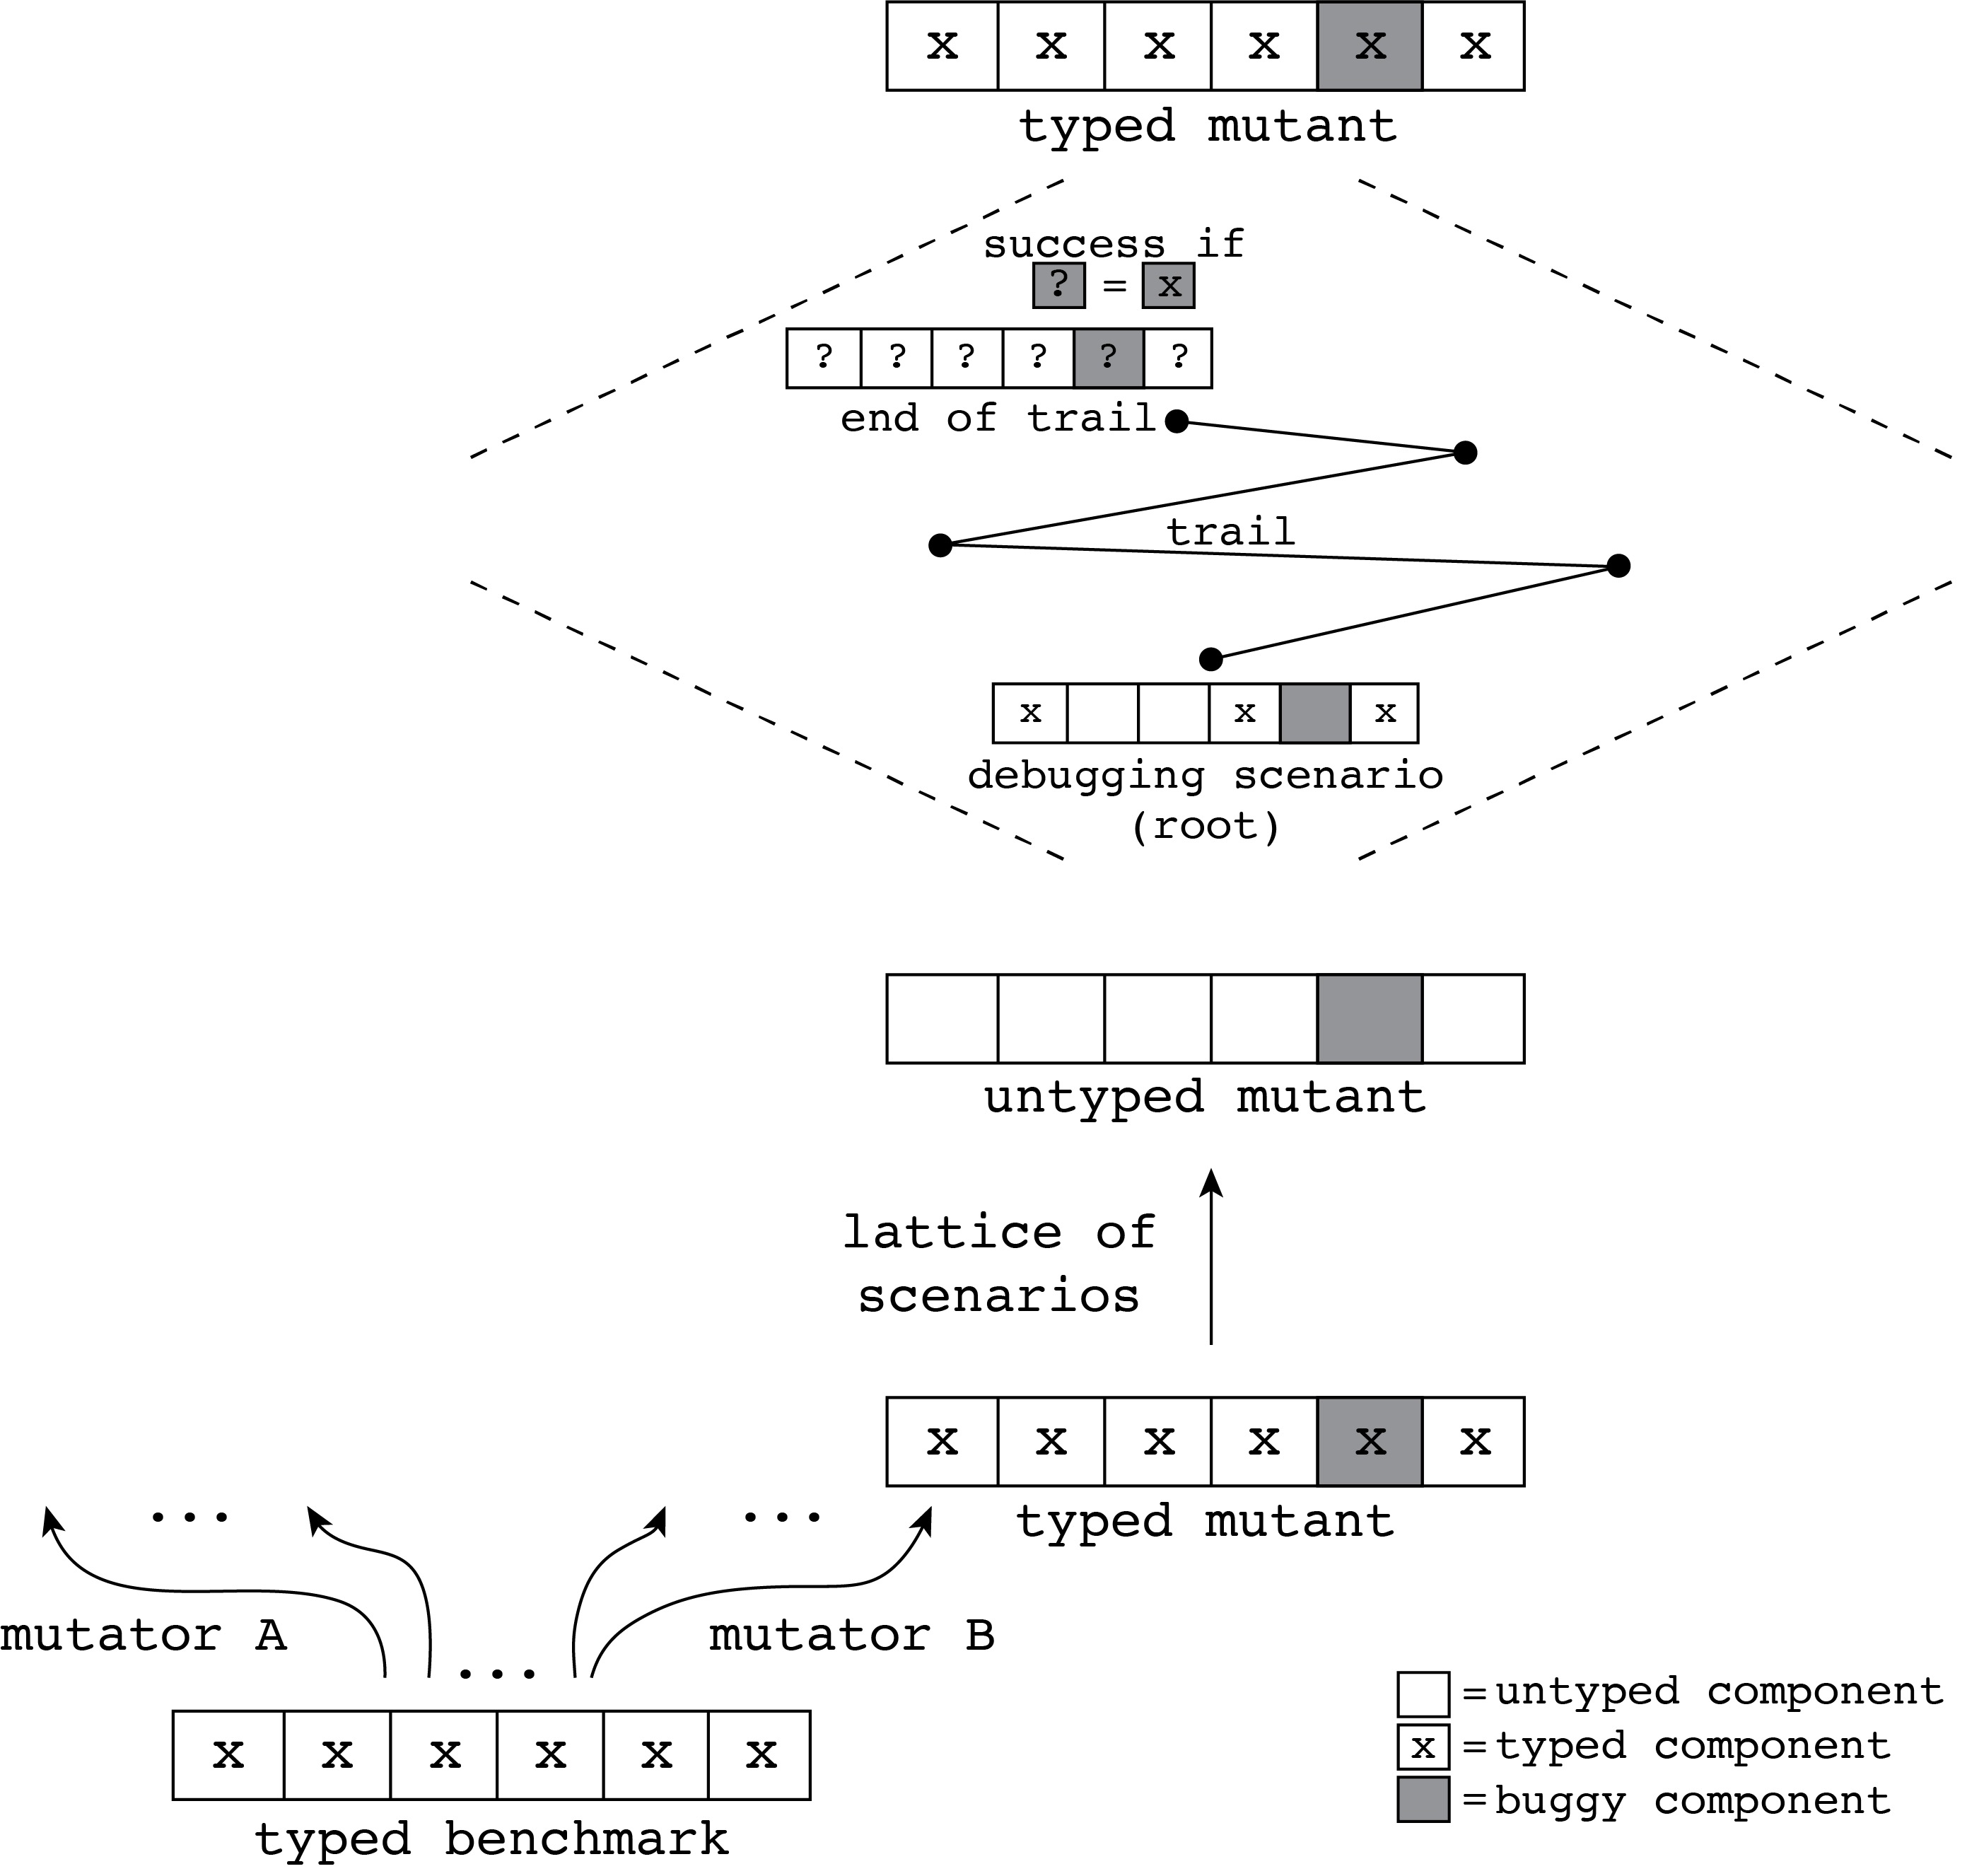
\includegraphics[width=\textwidth]{./Images/process}
  \caption{The experimental process for one mode of the rational
  programmer}
  \label{fig:process}
\end{figure}


\subsection{Programmer Effort}

In addition to successful and failure information for the various trails,  
our experiment  records the number of components a rational programmer 
has to type along each successful trail ($\lvert \conf_n \setminus \conf_0
\rvert$). We use this number as the metric for the effort 
of the rational programmer to debug the root scenario of each successful trail.  

Programmer effort can help shed some light to the relative effectiveness of the
three gradual typing systems. For example, consider a debugging scenario from  the
lattice of one of our mutants.  If the
scenario results in blame both under, for instance, the natural and transient semantics,
then the natural blame rational programmer and the two transient blame
rational programmers (all and firstborn) can compete to see which one
reaches an ill-typed scenarion with less effort. In
general, the effort of trails of different modes that have the same
root is a point of comparison for the effectiveness of these
modes even if the modes correspond to different gradual typing systems.
Unfortunately, statistically speaking, such comparisons between two modes do not generalize 
beyond the successful trails with common roots in our experiments.
Still they allow us to quantify the difference between the modes of the rational
programmers and thus the different blame assignment strategies  for the specific
debugging scenarios we analyze in our experiment.
